\documentclass[11pt]{article}

\usepackage[margin=0.82in]{geometry}
\usepackage[T1]{fontenc}
\usepackage[utf8]{inputenc}
\usepackage{lmodern}
\usepackage{amsmath,amssymb,mathtools}
\usepackage{array}
\usepackage{booktabs}
\usepackage{enumitem}
\usepackage{graphicx}
\usepackage{xcolor}
\usepackage{hyperref}
\usepackage{tikz}
\usepackage[most]{tcolorbox}
\usepackage{longtable}
\usepackage{multicol}
\usetikzlibrary{arrows.meta,positioning,shapes.geometric,calc,fit}

\hypersetup{
  colorlinks=true,
  linkcolor=blue!55!black,
  urlcolor=blue!55!black,
  citecolor=blue!55!black
}

\setlist[itemize]{topsep=2pt,itemsep=2pt,leftmargin=*}
\setlist[enumerate]{topsep=2pt,itemsep=2pt,leftmargin=*}
\renewcommand{\arraystretch}{1.18}

\definecolor{BOBlue}{RGB}{0,64,128}
\definecolor{SoftBlue}{RGB}{235,244,255}
\definecolor{SoftGray}{RGB}{246,246,246}
\definecolor{SoftGreen}{RGB}{238,248,239}
\definecolor{SoftRed}{RGB}{255,241,241}
\definecolor{SoftYellow}{RGB}{255,250,232}

\newtcolorbox{keybox}[1]{
  enhanced,
  breakable,
  colback=SoftBlue,
  colframe=BOBlue,
  title=\textbf{#1},
  arc=2mm,
  boxrule=0.6pt
}

\newtcolorbox{answerbox}[1]{
  enhanced,
  breakable,
  colback=SoftGreen,
  colframe=green!40!black,
  title=\textbf{#1},
  arc=2mm,
  boxrule=0.6pt
}

\newtcolorbox{warningbox}[1]{
  enhanced,
  breakable,
  colback=SoftRed,
  colframe=red!55!black,
  title=\textbf{#1},
  arc=2mm,
  boxrule=0.6pt
}

\newtcolorbox{examplebox}[1]{
  enhanced,
  breakable,
  colback=SoftYellow,
  colframe=orange!65!black,
  title=\textbf{#1},
  arc=2mm,
  boxrule=0.6pt
}

\newcommand{\principle}[1]{\textbf{\textcolor{BOBlue}{#1}}}
\newcommand{\question}[1]{\paragraph{Question.} #1}
\newcommand{\stronganswer}[1]{\paragraph{Strong answer.} #1}
\newcommand{\dd}{\mathrm{d}}
\newcommand{\Hz}{\mathrm{Hz}}
\newcommand{\mV}{\mathrm{mV}}
\newcommand{\V}{\mathrm{V}}
\newcommand{\mA}{\mathrm{mA}}
\newcommand{\psiu}{\mathrm{psi}}

\title{\textbf{Blue Origin Panel Interview Preparation Guide -- Updated Expanded Edition}\\
\large Data Acquisition and Controls Engineer II -- New Glenn, R66427}
\author{Expanded Technical and Behavioral Study Notes}
\date{\today}

\begin{document}
\maketitle

\begin{abstract}
This expanded edition explains the topics previously listed as preparation
items. It is written as both an interview guide and a compact technical
reference. It covers sensor selection, signal conditioning, ADCs, sampling,
grounding, controls, safety, Python software architecture, NI/DAQmx concepts,
data processing, databases, electrical troubleshooting, commissioning, system
design, and behavioral interview answers. Examples, equations, and figures are
included where they help explain the engineering reasoning.
\end{abstract}

\begin{keybox}{Core interview message}
``I can translate test objectives into a safe, traceable, and maintainable
measurement-and-control system--from sensor selection and signal conditioning
through acquisition, automated control, data validation, post-processing, and
engineering review.''
\end{keybox}

\tableofcontents
\newpage

\section{How to Think About the Role}

\subsection{The end-to-end test system}
A Data Acquisition and Controls Engineer does not only connect sensors or write
scripts. The engineer owns the chain by which a physical event becomes trusted
engineering evidence. A complete answer should connect hardware, software,
safety, data integrity, and review.

\begin{center}
\resizebox{0.98\linewidth}{!}{%
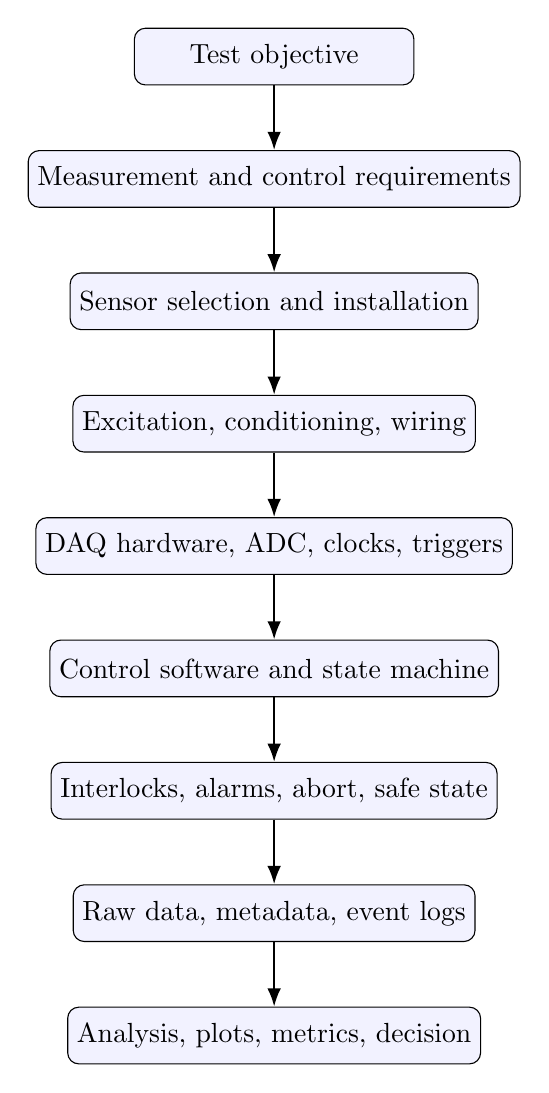
\begin{tikzpicture}[node distance=0.82cm,>=Latex]
  \tikzstyle{block}=[draw,rounded corners,align=center,minimum width=3.55cm,minimum height=0.72cm,fill=blue!5]
  \node[block] (obj) {Test objective};
  \node[block,below=of obj] (req) {Measurement and control requirements};
  \node[block,below=of req] (sensor) {Sensor selection and installation};
  \node[block,below=of sensor] (signal) {Excitation, conditioning, wiring};
  \node[block,below=of signal] (daq) {DAQ hardware, ADC, clocks, triggers};
  \node[block,below=of daq] (control) {Control software and state machine};
  \node[block,below=of control] (safe) {Interlocks, alarms, abort, safe state};
  \node[block,below=of safe] (store) {Raw data, metadata, event logs};
  \node[block,below=of store] (analysis) {Analysis, plots, metrics, decision};
  \foreach \a/\b in {obj/req,req/sensor,sensor/signal,signal/daq,daq/control,control/safe,safe/store,store/analysis}
    \draw[->,thick] (\a) -- (\b);
\end{tikzpicture}}
\end{center}

\subsection{What an Engineer II should demonstrate}
At this level, the panel will likely expect:
\begin{itemize}
  \item Independent execution on scoped systems.
  \item Ability to identify incomplete requirements.
  \item Defensible tradeoffs involving safety, data quality, schedule, cost, and maintainability.
  \item Troubleshooting across mechanical, electrical, controls, software, and data boundaries.
  \item Clear communication to test operations, design engineering, controls, analysis, and management.
  \item Respect for formal reviews, calibration, configuration control, and safety authority.
\end{itemize}

\section{Sensor Selection: Detailed Explanations}

\subsection{Measurement range}
The measurement range is the minimum and maximum value the sensor can measure
within its specified performance. Selecting range is a tradeoff:
\begin{itemize}
  \item Too small: the sensor may saturate or be damaged during transient or fault conditions.
  \item Too large: the useful signal occupies a small part of the range, reducing practical resolution.
\end{itemize}

\begin{examplebox}{Pressure range example}
Nominal pressure is \(2000~\psi\), but transients may reach \(2600~\psi\).
A \(2000~\psi\) transducer is inappropriate because it may saturate during
credible operation. A \(3000~\psi\) transducer may be reasonable if proof
pressure, burst pressure, accuracy, and resolution are acceptable.
\end{examplebox}

\subsection{Accuracy versus precision}
\textbf{Accuracy} is closeness to the true value. \textbf{Precision} is
repeatability or tight clustering of repeated readings. A precise sensor can be
inaccurate if it has an offset; an accurate system should be both calibrated and
repeatable enough for the decision being made.

\begin{center}
\resizebox{0.88\linewidth}{!}{%
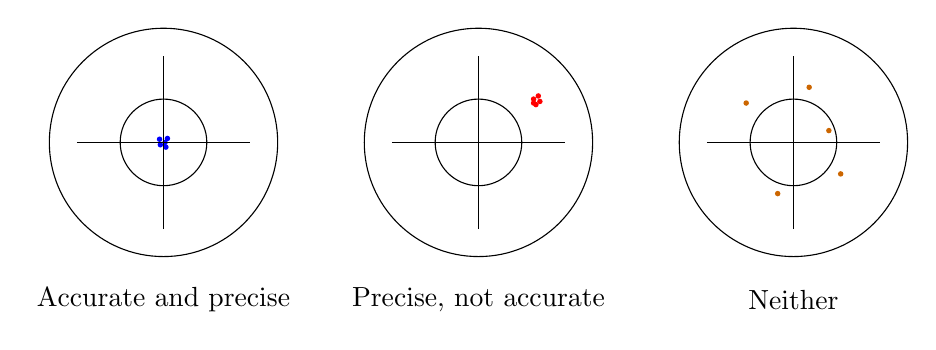
\begin{tikzpicture}
  \tikzstyle{target}=[circle,draw,minimum size=2.9cm]
  \node[target] (a) at (0,0) {};
  \node at (0,-2) {Accurate and precise};
  \foreach \p in {(0.05,0.05),(-0.05,0.04),(0.03,-0.06),(-0.04,-0.03),(0.02,0.0)}
    \fill[blue] \p circle (0.035);
  \node[target] (b) at (4,0) {};
  \node at (4,-2) {Precise, not accurate};
  \foreach \p in {(4.7,0.55),(4.78,0.52),(4.73,0.48),(4.76,0.59),(4.70,0.50)}
    \fill[red] \p circle (0.035);
  \node[target] (c) at (8,0) {};
  \node at (8,-2) {Neither};
  \foreach \p in {(7.4,0.5),(8.6,-0.4),(8.2,0.7),(7.8,-0.65),(8.45,0.15)}
    \fill[orange!80!black] \p circle (0.035);
  \foreach \x in {0,4,8} {
    \draw (\x-1.1,0) -- (\x+1.1,0);
    \draw (\x,-1.1) -- (\x,1.1);
    \draw (\x,0) circle (0.55);
  }
\end{tikzpicture}}
\end{center}

\subsection{Sensitivity}
Sensitivity is output change per input change. For example, a pressure sensor
may output \(10~\mV/\V\) at full scale or \(5~\V\) over a \(0\) to
\(3000~\psi\) range. High sensitivity is useful when small changes must be
resolved, but it does not guarantee accuracy.

\subsection{Resolution}
Resolution is the smallest distinguishable increment. It is affected by the
sensor, signal conditioner, ADC span, noise, and digital representation.

\begin{examplebox}{Resolution example}
If a \(0\) to \(3000~\psi\) transducer is digitized over a \(0\) to \(10~\V\)
range using a 16-bit ADC, the ideal pressure step is approximately
\[
\Delta P = \frac{3000~\psi}{2^{16}} \approx 0.046~\psi.
\]
This is ideal resolution, not total accuracy. Noise and calibration can make the
effective resolution worse.
\end{examplebox}

\subsection{Linearity}
Linearity describes how closely sensor output follows a straight-line
relationship with input. Nonlinearity is often specified as a percentage of full
scale. A nonlinear sensor can still be useful if a calibration curve or
linearization model is applied.

\subsection{Hysteresis}
Hysteresis means the output depends on whether the input is approached from
above or below. For example, a pressure transducer may read slightly differently
at \(1000~\psi\) during pressurization than during depressurization. This matters
when acceptance criteria are tight or when load/unload cycles are evaluated.

\subsection{Repeatability}
Repeatability is the ability to return to the same reading under the same
conditions. In test operations, repeatability affects confidence that trends are
caused by hardware behavior rather than measurement instability.

\subsection{Drift}
Drift is slow change in sensor output over time, temperature, or usage. Zero
drift shifts the output at no input; span drift changes sensitivity. Drift is
managed with warmup periods, calibration intervals, temperature compensation,
and pre/post-test zero checks.

\subsection{Bandwidth and dynamic response}
Bandwidth is the frequency range over which the sensor accurately follows input.
A slow sensor can attenuate or phase-shift fast transients.

For a first-order sensor with time constant \(\tau\), the approximate cutoff
frequency is:
\[
f_c = \frac{1}{2\pi \tau}.
\]

\begin{examplebox}{Dynamic response example}
If a temperature probe has \(\tau = 0.5~\mathrm{s}\), then
\[
f_c \approx \frac{1}{2\pi(0.5)} \approx 0.32~\Hz.
\]
It is suitable for slow thermal trends but not for fast thermal transients.
\end{examplebox}

\subsection{Environmental rating}
Sensors must survive temperature, vibration, humidity, vacuum, chemical
exposure, pressure media, electromagnetic environment, and mechanical shock.
Environmental compatibility is especially important in propulsion and
pressurized-fluid testing.

\subsection{Calibration}
Calibration compares a sensor chain to a known standard. Good calibration
practice includes:
\begin{itemize}
  \item Traceability to a standard.
  \item Calibration date and due date.
  \item As-found and as-left data.
  \item Calibration coefficients or curves.
  \item Uncertainty statement.
  \item Configuration control so the correct coefficients are used in software.
\end{itemize}

\subsection{Over-range protection}
Over-range protection prevents sensor damage or unsafe behavior if input exceeds
normal range. It may include mechanical stops, relief valves, snubbers, input
clamps, fuses, current limiting, proof pressure margins, or software alarms.

\subsection{Mounting effects and sensor loading}
The sensor can disturb the system being measured. Examples:
\begin{itemize}
  \item A pressure tap with long tubing can introduce resonance or damping.
  \item A thermocouple bead with large mass can slow response.
  \item A voltmeter with low input impedance can load a circuit.
  \item A load cell installed with side loads can produce erroneous readings.
\end{itemize}

\section{Important Sensor Types}

\subsection{Pressure transducers}
\subsubsection{Absolute, gauge, sealed gauge, and differential}
\begin{itemize}
  \item \textbf{Absolute pressure} is measured relative to vacuum.
  \item \textbf{Gauge pressure} is measured relative to local atmosphere.
  \item \textbf{Sealed gauge} is referenced to a sealed reference pressure.
  \item \textbf{Differential pressure} measures the difference between two ports.
\end{itemize}

\[
P_{\mathrm{abs}} = P_{\mathrm{gauge}} + P_{\mathrm{atm}}.
\]

\subsubsection{Voltage and current outputs}
Common outputs include \(0\) to \(5~\V\), \(0\) to \(10~\V\), millivolt bridge
outputs, and \(4\) to \(20~\mA\). Current loops are often preferred for long
cables and noisy environments.

\subsubsection{Proof and burst pressure}
Proof pressure is the pressure the device can withstand without permanent
performance change. Burst pressure is the pressure at which containment may
fail. A credible transient must remain below appropriate limits with margin.

\subsubsection{Tubing and mounting effects}
Pressure tubing adds volume, resistance, and compliance. It can act as a low-pass
filter or resonator. If the measurement objective is fast transient pressure,
mount the sensor close to the source and verify dynamic response.

\subsection{Thermocouples}
\subsubsection{Seebeck effect}
A thermocouple generates a voltage because two dissimilar metals form junctions
at different temperatures. The output is small, often tens of microvolts per
degree Celsius.

\subsubsection{Cold-junction compensation}
Thermocouple voltage depends on the temperature difference between the sensing
junction and the reference junction. Cold-junction compensation measures the
reference junction temperature and mathematically compensates the reading.

\[
T_{\mathrm{hot}} = f^{-1}\left(V_{\mathrm{TC}} + f(T_{\mathrm{cold}})\right).
\]

\subsubsection{Grounded versus ungrounded junctions}
Grounded thermocouples have faster response but can create ground-loop or
common-mode problems. Ungrounded thermocouples are slower but electrically
isolated from the sheath.

\subsection{RTDs}
An RTD changes resistance with temperature. Platinum RTDs are common because they
are stable and accurate.

\[
R(T) \approx R_0(1+\alpha T)
\]
near a limited temperature range, where \(R_0\) is resistance at \(0^\circ C\)
and \(\alpha\) is the temperature coefficient.

\subsubsection{Two-, three-, and four-wire RTDs}
\begin{itemize}
  \item \textbf{Two-wire}: simplest, but lead resistance adds error.
  \item \textbf{Three-wire}: compensates lead resistance if lead wires are matched.
  \item \textbf{Four-wire}: best accuracy; separate excitation and sense leads.
\end{itemize}

\subsection{Load cells and strain gauges}
\subsubsection{Wheatstone bridge}
Strain gauges often use a Wheatstone bridge. A full bridge uses four active arms;
a half bridge uses two; a quarter bridge uses one active gauge and completion
resistors.

\begin{center}
\begin{tikzpicture}[>=Latex]
  \node (top) at (0,2) {};
  \node (left) at (-1.6,0) {};
  \node (right) at (1.6,0) {};
  \node (bot) at (0,-2) {};
  \draw (top) -- node[left] {$R_1$} (left) -- node[left] {$R_2$} (bot);
  \draw (top) -- node[right] {$R_3$} (right) -- node[right] {$R_4$} (bot);
  \draw[->] (-2.6,0) -- (left) node[midway,above] {$V_o-$};
  \draw[->] (2.6,0) -- (right) node[midway,above] {$V_o+$};
  \draw[->] (0,2.8) -- (top) node[midway,right] {$+V_{ex}$};
  \draw[->] (0,-2.8) -- (bot) node[midway,right] {$-V_{ex}$};
\end{tikzpicture}
\end{center}

For a balanced bridge,
\[
\frac{R_1}{R_2} = \frac{R_3}{R_4}, \qquad V_o = 0.
\]
Strain changes resistance and produces a small differential output.

\subsubsection{mV/V sensitivity}
A load cell rated \(2~\mV/\V\) produces \(2~\mV\) per volt of excitation at full
scale. With \(10~\V\) excitation, full-scale output is:
\[
V_{\mathrm{FS}} = 2~\frac{\mV}{\V}\times 10~\V = 20~\mV.
\]
This small signal requires differential low-noise amplification.

\subsubsection{Shunt calibration}
Shunt calibration places a known resistor across one bridge arm to simulate a
known strain/load. It checks wiring, excitation, bridge completion, and scaling,
but it does not replace mechanical calibration of the full load path.

\section{Signal Conditioning: Expanded Explanations}

\subsection{Amplification}
Amplification increases signal amplitude before digitization. It is useful when
the sensor output is small compared with ADC input span.

\[
V_{\mathrm{out}} = G V_{\mathrm{in}},
\]
where \(G\) is gain.

\begin{examplebox}{Amplifying a load-cell signal}
A load cell produces \(0\) to \(20~\mV\). If the ADC range is \(0\) to \(10~\V\),
the signal uses only \(0.2\%\) of the ADC span. A gain of \(250\) maps
\(20~\mV\) to \(5~\V\), greatly improving usable resolution. The amplifier must
not saturate during overloads.
\end{examplebox}

\subsection{Attenuation}
Attenuation reduces signal amplitude so it fits within the measurement input
range. It is common for high-voltage measurements.

For a resistor divider:
\[
V_{\mathrm{out}} = V_{\mathrm{in}}\frac{R_2}{R_1+R_2}.
\]

\begin{examplebox}{Voltage divider example}
To measure \(100~\V\) with a \(10~\V\) ADC, use a 10:1 divider. If
\(R_1=90~\mathrm{k}\Omega\) and \(R_2=10~\mathrm{k}\Omega\),
\[
V_{\mathrm{out}}=100\frac{10}{90+10}=10~\V.
\]
Check resistor power, tolerance, temperature coefficient, and isolation.
\end{examplebox}

\subsection{Filtering}
Filtering removes unwanted frequency content. Filters can be analog or digital.
Analog filtering before the ADC is required for anti-alias protection.

\subsubsection{Low-pass filter}
A first-order RC low-pass filter has cutoff:
\[
f_c = \frac{1}{2\pi RC}.
\]
Signals below \(f_c\) mostly pass; signals above \(f_c\) are attenuated.

\subsubsection{High-pass, band-pass, and notch filters}
\begin{itemize}
  \item \textbf{High-pass}: removes slow drift or DC offset.
  \item \textbf{Band-pass}: isolates a frequency band.
  \item \textbf{Notch}: rejects a narrow frequency, such as 60 Hz interference.
\end{itemize}

\subsection{Anti-alias filtering}
Aliasing occurs when frequency content above half the sample rate appears as a
false lower-frequency signal after sampling. If sample rate is \(f_s\), the
Nyquist frequency is:
\[
f_N = \frac{f_s}{2}.
\]
Analog content above \(f_N\) must be attenuated before digitization.

\begin{center}
\resizebox{0.93\linewidth}{!}{%
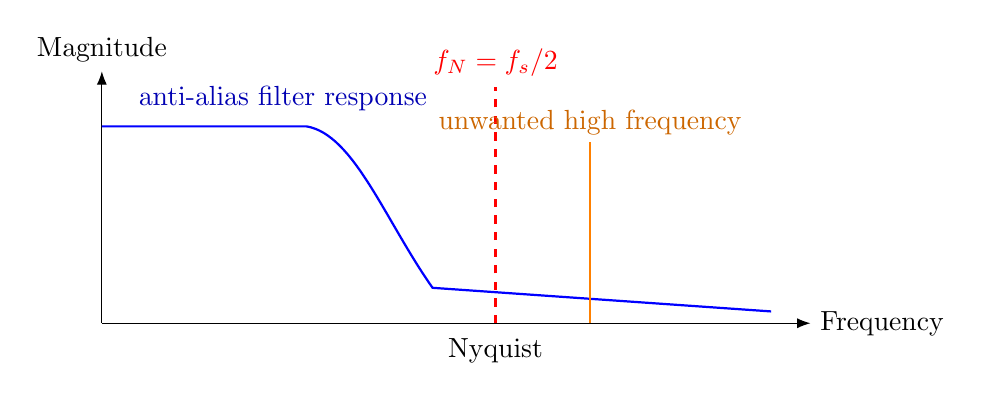
\begin{tikzpicture}[>=Latex]
  \draw[->] (0,0) -- (9,0) node[right] {Frequency};
  \draw[->] (0,0) -- (0,3.2) node[above] {Magnitude};
  \draw[thick,blue] (0,2.5) -- (2.6,2.5) .. controls (3.2,2.4) and (3.6,1.3) .. (4.2,0.45) -- (8.5,0.15);
  \draw[dashed,red,thick] (5,0) -- (5,3) node[above] {$f_N=f_s/2$};
  \draw[orange,thick] (6.2,0) -- (6.2,2.3);
  \node[orange!80!black] at (6.2,2.55) {unwanted high frequency};
  \node[blue!70!black] at (2.3,2.85) {anti-alias filter response};
  \node at (5,-0.35) {Nyquist};
\end{tikzpicture}}
\end{center}

\subsection{Isolation}
Isolation breaks direct electrical connection between two parts of a system
while allowing signal transfer. It protects people and equipment, reduces ground
loops, and handles large common-mode voltages. Isolation may be optical,
magnetic, capacitive, transformer-based, or implemented with isolated DAQ
modules.

\begin{examplebox}{Isolation example}
A sensor mounted on equipment with a different ground potential may exceed the
DAQ common-mode range. An isolated signal conditioner allows the sensor side and
DAQ side to float relative to one another within the isolation rating.
\end{examplebox}

\subsection{Sensor excitation}
Some sensors require external power or excitation:
\begin{itemize}
  \item Strain gauges and load cells require bridge excitation.
  \item RTDs require a controlled current or voltage.
  \item IEPE accelerometers require constant-current excitation.
  \item Some pressure transducers require regulated DC supply.
\end{itemize}
Excitation stability directly affects measurement accuracy.

\subsection{Bridge completion}
Quarter-bridge strain gauges do not form a full Wheatstone bridge by themselves.
Bridge completion adds precision resistors to complete the bridge. The
completion network must be stable, low noise, and configured correctly for the
gauge resistance.

\subsection{Cold-junction compensation}
Cold-junction compensation is signal conditioning specific to thermocouples. The
DAQ must know the temperature at the reference junction, often where the
thermocouple wire connects to copper terminals. Without compensation, the
reported temperature can be biased by terminal-block temperature.

\subsection{Linearization}
Many sensors are nonlinear. Linearization converts raw voltage, current, or
resistance into engineering units using equations, lookup tables, or calibration
curves. Thermocouples, RTDs, and some flow meters commonly require
linearization.

\subsection{Current-to-voltage conversion}
DAQ analog inputs usually measure voltage, so a \(4\) to \(20~\mA\) current loop
often uses a precision shunt resistor:
\[
V = IR.
\]
With \(R=250~\Omega\),
\[
4~\mA \rightarrow 1~\V, \qquad 20~\mA \rightarrow 5~\V.
\]
Use precision resistors with suitable power rating and temperature coefficient.

\subsection{Differential versus single-ended measurements}
\begin{itemize}
  \item \textbf{Single-ended}: signal measured relative to a common reference.
  \item \textbf{Differential}: voltage measured between two input terminals.
\end{itemize}
Differential measurements reject noise common to both leads and are preferred for
low-level or long-cable signals.

\[
V_{\mathrm{meas}} = V_+ - V_-.
\]

\subsection{Common-mode voltage}
Common-mode voltage is the voltage shared by both differential inputs relative
to DAQ ground:
\[
V_{\mathrm{CM}} = \frac{V_+ + V_-}{2}.
\]
Even if \(V_+ - V_-\) is small, a large common-mode voltage can exceed the
input specification and cause saturation or damage.

\subsection{Common-mode rejection}
Common-mode rejection ratio (CMRR) measures how well an amplifier rejects common
noise:
\[
\mathrm{CMRR}_{dB}=20\log_{10}\left(\frac{A_d}{A_{cm}}\right),
\]
where \(A_d\) is differential gain and \(A_{cm}\) is common-mode gain. Higher is
better.

\subsection{Input impedance}
Input impedance is the effective resistance/capacitance seen by the signal
source. Low input impedance can load the sensor and change the measured value.
A voltage measurement system should usually have much higher input impedance
than the source impedance.

\subsection{Ground loops}
A ground loop occurs when two or more ground paths create circulating current.
This current can add noise or offset to low-level measurements. It is common
when sensors, DAQ systems, power supplies, and test hardware are grounded at
different points.

\subsection{Shielding and cable routing}
Shields intercept electric-field noise; twisted pairs reduce magnetic pickup;
separation from high-current or switching cables reduces coupling. Shield
termination strategy depends on frequency, equipment bonding, isolation, and
manufacturer guidance.

\section{Sampling, Timing, and ADCs}

\subsection{Sampling rate}
Sampling rate \(f_s\) is samples per second. It must be high enough to capture
the signal of interest, support control timing, and allow anti-alias filtering.
A practical rule is often \(5\) to \(10\) times the highest frequency of
interest for time-domain shape, but final selection depends on the objective.

\subsection{Nyquist criterion}
The theoretical minimum sampling rate for a maximum signal frequency \(f_{\max}\)
is:
\[
f_s > 2f_{\max}.
\]
In practice, choose a higher rate to allow filter roll-off and transient
fidelity.

\subsection{Aliasing equation}
A sinusoid at frequency \(f\) sampled at \(f_s\) can appear at an alias
frequency:
\[
f_{\mathrm{alias}} = |f - kf_s|,
\]
for an integer \(k\) chosen so the result falls below \(f_s/2\).

\begin{examplebox}{Aliasing example}
If \(f_s=1000~\Hz\) and unwanted vibration is at \(900~\Hz\), it may appear as a
\(100~\Hz\) signal because \(900\) is \(100~\Hz\) away from \(1000~\Hz\). Without
an analog anti-alias filter, the data may falsely suggest a 100 Hz physical
phenomenon.
\end{examplebox}

\subsection{ADC quantization}
For an \(N\)-bit ADC with full-scale span \(V_{\mathrm{span}}\):
\[
\Delta V = \frac{V_{\mathrm{span}}}{2^N}.
\]
If the input range is \(-10\) to \(+10~\V\), then \(V_{\mathrm{span}}=20~\V\).

\begin{examplebox}{16-bit ADC example}
\[
\Delta V = \frac{20~\V}{65536} \approx 305~\mu\V.
\]
If a sensor scaling is \(300~\psi/\V\), the ideal pressure step is:
\[
305~\mu\V \times 300~\frac{\psi}{\V} \approx 0.0915~\psi.
\]
\end{examplebox}

\subsection{Effective number of bits}
Noise reduces useful resolution. Effective number of bits (ENOB) describes
actual performance after noise and distortion:
\[
\mathrm{ENOB} \approx \frac{\mathrm{SNR}_{dB}-1.76}{6.02}.
\]
A 16-bit ADC may behave like a 13- or 14-bit system if noise is significant.

\subsection{Synchronization across channels}
Channels may be sampled simultaneously, multiplexed through one ADC, or acquired
by separate devices. Time alignment depends on shared clocks, triggers, cable
delays, filter delays, and timestamp strategy. For fast transients, hardware
synchronization is preferable to software timestamps.

\subsection{Deterministic versus non-deterministic acquisition}
Deterministic timing means operations occur within known timing bounds.
Hardware-timed DAQ and real-time controllers are more deterministic than normal
desktop operating systems. Non-deterministic processes can still be acceptable
for logging and user interfaces if they do not control safety-critical timing.

\section{Grounding, Shielding, and Noise Troubleshooting}

\subsection{Common sources of noise}
\begin{itemize}
  \item 50/60 Hz mains pickup.
  \item Motor drives and switching supplies.
  \item Radio-frequency interference.
  \item Ground loops.
  \item Poor shield termination.
  \item Long high-impedance sensor leads.
  \item Mechanical vibration or real physical pulsation.
  \item ADC range or amplifier saturation.
\end{itemize}

\subsection{Differential inputs and twisted pairs}
Twisted pairs help ensure external magnetic fields induce nearly equal voltage in
both conductors. A differential input then subtracts the two wires, rejecting
common noise.

\subsection{Single-point grounding}
Single-point grounding connects signal references at one controlled point to
avoid circulating currents. It is often useful for low-frequency systems, but it
is not universal. At high frequencies, cable shields may need multi-point bonding
to reduce RF impedance.

\subsection{Shield termination}
Possible strategies include one-end termination, both-end termination, capacitive
termination, or chassis 360-degree termination. The correct choice depends on
noise frequency, safety bonding, isolation, equipment instructions, and whether
the shield carries fault current.

\subsection{Troubleshooting method}
Use a disciplined process:
\begin{enumerate}
  \item Make the system safe.
  \item Identify affected channels and conditions.
  \item Look at raw data and spectrum if possible.
  \item Correlate noise with pumps, valves, power supplies, or motion.
  \item Inject known signals at successive points in the chain.
  \item Change one variable at a time.
  \item Document the result and root cause.
\end{enumerate}

\question{A pressure measurement is stable when the pump is off but noisy when the pump starts.}
\stronganswer{Treat both physical and electrical causes as plausible. The pump
could create real pressure ripple, mechanical vibration, electromagnetic
interference, ground current, or signal-conditioner saturation. Compare nearby
pressure sensors, review raw and filtered data, check frequency correlation with
pump speed or drive switching, inspect cable routing, verify shield continuity,
measure at the sensor and at the DAQ, and substitute a known signal. Do not
filter away the signal until you know whether it is noise or real pressure
behavior.}

\section{Controls and Automated Test Operations}

\subsection{Open-loop versus closed-loop control}
\textbf{Open-loop control} commands an actuator without using measured feedback.
Example: open a valve to 30 percent for 10 seconds.

\textbf{Closed-loop control} compares measured output to a setpoint and adjusts
the actuator to reduce error.
\[
e(t)=r(t)-y(t),
\]
where \(r(t)\) is setpoint and \(y(t)\) is measured output.

\subsection{PID control}
A PID controller computes:
\[
u(t)=K_p e(t)+K_i\int e(t)\dd t+K_d\frac{\dd e(t)}{\dd t}.
\]
\begin{itemize}
  \item \(K_p\): proportional response to current error.
  \item \(K_i\): integral response to accumulated error.
  \item \(K_d\): derivative response to rate of error change.
\end{itemize}

\subsection{Overshoot and settling time}
Overshoot is how far the response exceeds the target. Settling time is how long
it takes to remain within a specified band around the setpoint. In pressure
testing, excessive overshoot can violate limits; slow settling can waste test
time or invalidate hold intervals.

\subsection{Sensor delay}
Delay adds phase lag and can destabilize feedback loops. If a pressure sensor,
filter, or communication path delays the measurement, the controller may react
to old information.

\subsection{Actuator saturation}
Saturation occurs when the controller asks for more actuator authority than is
available, such as a valve command below 0 percent or above 100 percent. If the
integrator continues accumulating error during saturation, windup occurs.

\subsection{Integrator windup and anti-windup}
Integrator windup causes overshoot and slow recovery after saturation. Anti-windup
methods include clamping the integrator, back-calculation, conditional
integration, and resetting during mode changes.

\subsection{Rate limiting and setpoint ramping}
Rate limiting constrains how quickly commands or setpoints change. Setpoint
ramping prevents step commands from causing unsafe transients.
\[
r_{k+1}=r_k+\mathrm{clip}(r_{\mathrm{target}}-r_k,\,-R\Delta t,\,R\Delta t).
\]

\subsection{Discrete-time implementation}
Digital controllers update at sample time \(T_s\). Integral and derivative terms
must be implemented with correct timing:
\[
I_k = I_{k-1}+K_i e_k T_s,
\]
\[
D_k = K_d\frac{e_k-e_{k-1}}{T_s}.
\]
Incorrect \(T_s\) is a common source of unstable control behavior.

\subsection{State machines}
Test automation should use explicit states rather than a long unstructured
script. Each state has entry criteria, actions, exit criteria, timeouts, alarms,
and abort transitions.

\begin{center}
\resizebox{0.96\linewidth}{!}{%
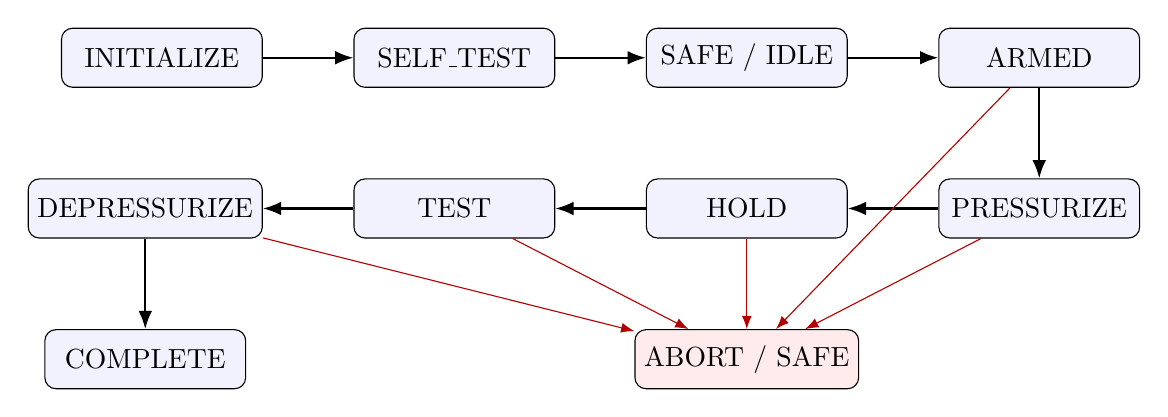
\begin{tikzpicture}[node distance=1.15cm,>=Latex]
  \tikzstyle{state}=[draw,rounded corners,align=center,minimum width=2.55cm,minimum height=0.75cm,fill=blue!5]
  \node[state] (init) {INITIALIZE};
  \node[state,right=of init] (self) {SELF\_TEST};
  \node[state,right=of self] (idle) {SAFE / IDLE};
  \node[state,right=of idle] (armed) {ARMED};
  \node[state,below=of armed] (press) {PRESSURIZE};
  \node[state,left=of press] (hold) {HOLD};
  \node[state,left=of hold] (test) {TEST};
  \node[state,left=of test] (dep) {DEPRESSURIZE};
  \node[state,below=of hold,fill=red!8] (abort) {ABORT / SAFE};
  \node[state,below=of dep] (complete) {COMPLETE};
  \foreach \a/\b in {init/self,self/idle,idle/armed,armed/press,press/hold,hold/test,test/dep,dep/complete}
    \draw[->,thick] (\a) -- (\b);
  \foreach \s in {armed,press,hold,test,dep}
    \draw[->,thin,red!70!black] (\s) -- (abort);
\end{tikzpicture}}
\end{center}

\subsection{Permissives, interlocks, and watchdogs}
\begin{itemize}
  \item \textbf{Permissive}: condition that must be true before an action is allowed.
  \item \textbf{Interlock}: protective logic that prevents or stops unsafe operation.
  \item \textbf{Watchdog}: mechanism that detects software or communication failure.
\end{itemize}

\subsection{Emergency shutdown and safe state}
Safe state is system-specific. It may mean venting pressure, closing supply
valves, opening relief paths, removing actuator power, or holding position. The
safe state must be defined by hazard analysis, not by convenience.

\question{A pressure-control loop oscillates around setpoint. What could cause it?}
\stronganswer{Possible causes include excessive proportional or integral gain,
process delay, sensor filtering, actuator deadband, valve stiction, saturation,
incorrect loop timing, noisy measurement, poor operating point, or unit errors.
Review setpoint, measurement, error, controller output, valve feedback, and
saturation flags before retuning.}

\section{Test Safety and Fault Management}

\subsection{Layered safety}
\begin{center}
\resizebox{0.95\linewidth}{!}{%
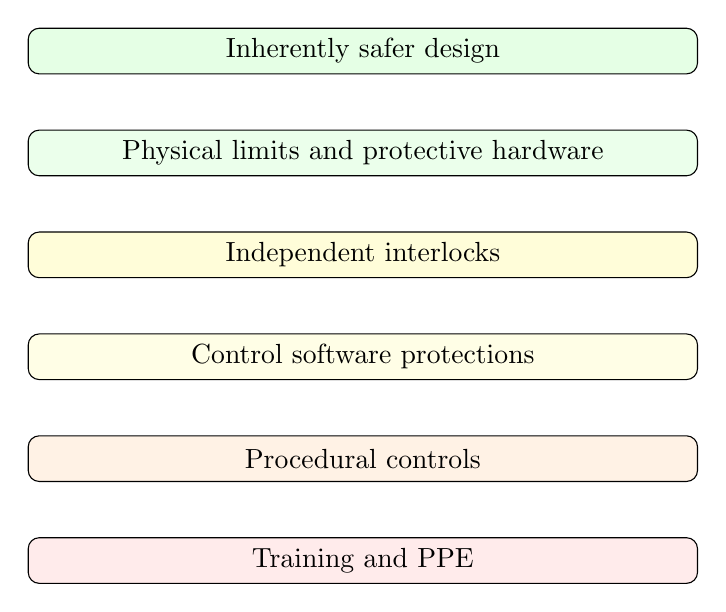
\begin{tikzpicture}[node distance=0.7cm,>=Latex]
  \tikzstyle{layer}=[draw,rounded corners,align=center,minimum width=8.5cm,minimum height=0.58cm]
  \node[layer,fill=green!10] (a) {Inherently safer design};
  \node[layer,below=of a,fill=green!8] (b) {Physical limits and protective hardware};
  \node[layer,below=of b,fill=yellow!15] (c) {Independent interlocks};
  \node[layer,below=of c,fill=yellow!10] (d) {Control software protections};
  \node[layer,below=of d,fill=orange!10] (e) {Procedural controls};
  \node[layer,below=of e,fill=red!8] (f) {Training and PPE};
\end{tikzpicture}}
\end{center}

\subsection{Fail-safe versus fail-operational}
\textbf{Fail-safe} means the system transitions to a safer condition after a
failure. \textbf{Fail-operational} means the system continues operating after a
failure, often with redundancy. Test stands commonly prioritize fail-safe
behavior unless stopping creates a greater hazard.

\subsection{Fault detection}
Fault detection can include limit checks, rate-of-change checks, sensor
disagreement, stale data detection, range checks, communication timeouts,
actuator feedback mismatch, and heartbeat/watchdog monitoring.

\subsection{Fault response}
Fault response should be defined before the test. Example responses:
\begin{itemize}
  \item Alarm only.
  \item Controlled hold.
  \item Controlled depressurization.
  \item Immediate abort.
  \item Hardware trip independent of software.
\end{itemize}

\question{What should the test stand do if communication with the controller is lost?}
\stronganswer{The response must come from hazard analysis. Do not assume that
holding the last command is safe. Outputs should transition predictably on
communication loss, watchdog timeout, application crash, or power loss. Critical
protection should remain effective even when supervisory software is unavailable.}

\section{Python Software Engineering for DAQ and Controls}

\subsection{Separation of concerns}
Good software separates hardware access, scaling, control logic, storage, user
interface, and analysis.

\begin{center}
\resizebox{0.94\linewidth}{!}{%
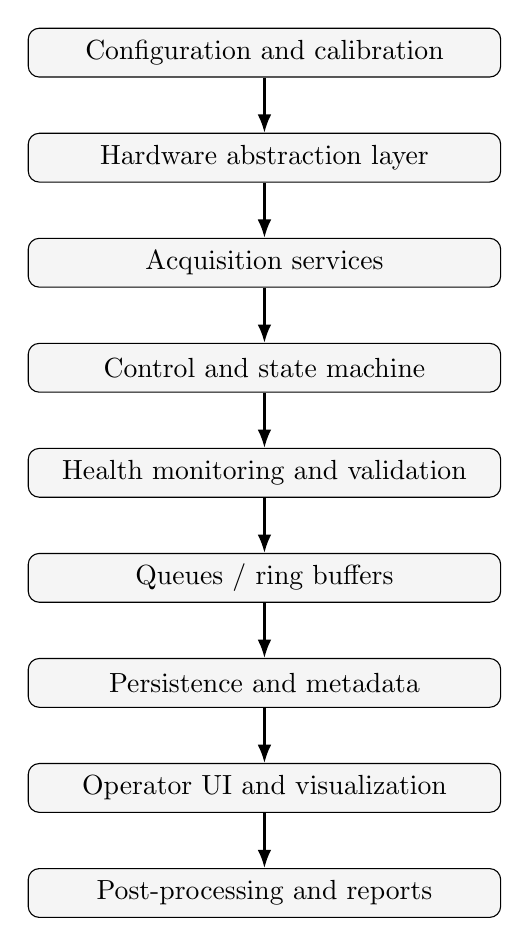
\begin{tikzpicture}[node distance=0.7cm,>=Latex]
  \tikzstyle{layer}=[draw,rounded corners,align=center,minimum width=6.0cm,minimum height=0.62cm,fill=gray!8]
  \node[layer] (config) {Configuration and calibration};
  \node[layer,below=of config] (hal) {Hardware abstraction layer};
  \node[layer,below=of hal] (acq) {Acquisition services};
  \node[layer,below=of acq] (control) {Control and state machine};
  \node[layer,below=of control] (health) {Health monitoring and validation};
  \node[layer,below=of health] (buffer) {Queues / ring buffers};
  \node[layer,below=of buffer] (persist) {Persistence and metadata};
  \node[layer,below=of persist] (ui) {Operator UI and visualization};
  \node[layer,below=of ui] (post) {Post-processing and reports};
  \foreach \a/\b in {config/hal,hal/acq,acq/control,control/health,health/buffer,buffer/persist,persist/ui,ui/post}
    \draw[->,thick] (\a) -- (\b);
\end{tikzpicture}}
\end{center}

\subsection{Classes and modules}
Use modules to group related functionality. Use classes for devices, channels,
configurations, and services when they have state and behavior. Avoid a single
large script that mixes hardware calls, scaling, plotting, and file writing.

\subsection{Type hints}
Type hints document intent and help tools detect mistakes:
\[
\texttt{def scale\_pressure(voltage: float, slope: float, offset: float) -> float}
\]
They are especially useful in DAQ code because units and data shapes matter.

\subsection{Exceptions}
Exceptions should represent exceptional conditions that the caller can handle or
surface. Do not silently catch all exceptions and continue as if data are valid.
For test systems, silent failure can create false confidence.

\subsection{Context managers}
Context managers ensure resources are opened and closed correctly:
\[
\texttt{with open(path, "wb") as f:}
\]
For DAQ, the same concept applies to hardware tasks: configure, start, stop, and
release resources deterministically.

\subsection{Logging}
Use structured logs for events, state transitions, commands, faults, software
versions, configuration IDs, and operator actions. Logs should support root-cause
analysis after a test.

\subsection{Unit testing and mocking hardware}
Unit tests verify scaling, state transitions, configuration validation, and
analysis calculations. Mock hardware allows tests without physical equipment.
However, mocked tests do not replace integration tests with real hardware.

\subsection{Concurrency: threads, processes, queues, async}
\begin{itemize}
  \item \textbf{Threads}: useful for I/O-bound tasks such as reading drivers and writing files.
  \item \textbf{Processes}: useful for CPU-heavy analysis that should bypass the Python GIL.
  \item \textbf{Queues}: safe handoff between acquisition, storage, and UI tasks.
  \item \textbf{Async I/O}: useful for many network or file I/O operations, less useful for CPU-heavy work.
\end{itemize}

\subsection{Bounded queues and backpressure}
Unbounded queues can hide failures until memory is exhausted. Bounded queues
force the design to define what happens if consumers fall behind.

\question{What happens if the disk writer falls behind?}
\stronganswer{Monitor queue depth and disk throughput. Warn early. Depending on
criticality, abort safely before data loss, reduce nonessential visualization,
or buffer for a bounded time. Do not silently drop samples unless that behavior
is explicitly allowed, logged, and visible to users.}

\subsection{Configuration management}
Configuration files should define channel names, hardware addresses, ranges,
scaling coefficients, calibration IDs, sample rates, alarms, and units. Store a
copy or hash of the configuration with each test dataset so analysis is
reproducible.

\section{NI Hardware, LabVIEW, and DAQmx}

\subsection{CompactDAQ versus PXI/PXIe}
\textbf{CompactDAQ} is modular and convenient for distributed or smaller test
systems. \textbf{PXI/PXIe} provides higher performance, tight synchronization,
and many specialized modules in a chassis architecture.

\subsection{Analog input and output}
Analog input measures continuous signals such as voltage, current, temperature,
pressure, strain, and acceleration. Analog output commands continuous values,
such as valve position or actuator setpoint.

\subsection{Digital I/O}
Digital inputs read discrete states such as limit switches, valve feedback,
interlock status, and emergency-stop contacts. Digital outputs command relays,
solenoids, enables, or indicators.

\subsection{Counter/timer channels}
Counters measure frequency, period, encoder position, pulse width, and event
counts. They are useful for flow meters, tachometers, encoders, and precise
timing.

\subsection{Hardware-timed acquisition}
Hardware timing uses a sample clock on the DAQ device. The host program reads
blocks of samples; it does not schedule each sample individually. This improves
sample interval consistency and synchronization.

\subsection{Software-timed acquisition}
Software timing relies on the host operating system to decide when each read or
write occurs. It is suitable for slow non-critical tasks but not for precise
sampling or control timing.

\subsection{Sample clocks and triggers}
A sample clock defines when samples are taken. A start trigger begins a task. A
reference trigger can capture data before and after an event. Shared clocks and
triggers synchronize multiple modules or devices.

\subsection{Buffered tasks}
Buffered acquisition stores samples in hardware or driver buffers before the
application reads them. Buffer sizing must handle expected latency without
overflow.

\subsection{Continuous versus finite sampling}
Finite sampling collects a specified number of samples. Continuous sampling runs
until stopped and requires the application to keep reading data fast enough.

\subsection{LabVIEW producer-consumer architecture}
A producer loop acquires data or handles events. A consumer loop processes,
displays, or writes data. Queues decouple timing so slow consumers do not block
time-critical producers.

\subsection{LabVIEW state machines}
LabVIEW state machines use cases or queued messages to transition between
states. The same engineering rules apply: explicit states, defined transitions,
timeouts, fault handling, and logging.

\section{Data Processing, Validation, and Visualization}

\subsection{Raw data preservation}
Never overwrite raw data with filtered or scaled-only values. Raw data allow
reanalysis if calibration, filtering, or requirements change.

\subsection{File integrity}
Use file size checks, checksums, complete headers, finalization flags, and
metadata validation to detect incomplete or corrupted files.

\subsection{Engineering-unit conversion}
Raw voltage or counts are converted to engineering units:
\[
y = mx+b
\]
for a linear sensor, or
\[
y = f(x)
\]
for a calibration curve. Always preserve units.

\subsection{Invalid and missing samples}
Invalid samples should be flagged, not silently filled. Missing data may be due
to sensor dropout, saturated ADC, dropped packets, file corruption, or intentional
test pauses.

\subsection{Time alignment}
Channels can be misaligned by separate clocks, multiplexing, filters, sensor
response, communication delays, or timestamp interpretation. Alignment should be
based on known timing architecture or identifiable physical events.

\subsection{Filtering in analysis}
Document filter type, order, cutoff, phase behavior, and whether it is causal or
zero-phase. Avoid using filters to make data look better without engineering
justification.

\subsection{Metrics and pass/fail}
A good report shows:
\begin{itemize}
  \item Metric value and units.
  \item Acceptance limit.
  \item Margin to limit.
  \item Data-quality status.
  \item Time interval used.
  \item Calibration and software versions.
\end{itemize}

\question{How would you determine whether a component passed a test?}
\stronganswer{Define acceptance criteria with the responsible engineering
authority. Identify exact channels and time intervals. Verify data quality.
Compute metrics with units and uncertainty. Report result, limit, margin,
quality flags, raw-data reference, configuration, calibration, and analysis-code
version. If required data are invalid, report indeterminate rather than false
pass or false fail.}

\section{Databases and Data Architecture}

\subsection{Raw waveform storage versus metadata storage}
Large waveform data are often stored in files such as TDMS, HDF5, Parquet, or
binary formats. Metadata are stored in a database for searchability. This avoids
putting huge time-series arrays directly into relational tables while preserving
traceability.

\subsection{Relational databases}
Relational databases store structured tables with relationships. Example tables:
Tests, TestArticles, Channels, Calibrations, Configurations, Operators, and
Results.

\subsection{Time-series databases}
Time-series databases optimize queries over timestamped data. They are useful
for long-duration monitoring but may not replace immutable raw files for
qualification evidence.

\subsection{Schema design}
A schema should answer: What was tested? When? By whom? With which procedure,
software, DAQ configuration, calibration, hardware serial numbers, and
acceptance limits?

\subsection{Checksums}
A checksum or hash detects file changes:
\[
\mathrm{hash} = H(\mathrm{file~bytes}).
\]
Store hashes with metadata to detect corruption or unintended modification.

\subsection{Calibration traceability}
Each channel should link to the calibration record used during the test. If a
calibration expires or is later found invalid, affected tests can be identified.

\section{Electrical Schematics and Wiring Diagrams}

\subsection{Power distribution}
Understand source, breakers, fuses, disconnects, power supplies, voltage rails,
returns, and protective earth. Confirm voltage rating and current capacity.

\subsection{Relays and contactors}
Relays switch lower-power circuits; contactors switch higher-power loads.
Coil voltage, contact rating, normally open/normally closed behavior, and
flyback suppression matter.

\subsection{Terminal blocks and connector pinouts}
Terminal blocks provide wiring transition points. Connector pinouts identify
signals, returns, shields, and spare pins. Wrong pinouts are common integration
failures.

\subsection{Normally open and normally closed contacts}
A normally closed safety contact is closed in the normal safe condition and opens
on trip or wire break. This can make some faults detectable.

\subsection{Return paths}
Every signal requires a return path. Missing or shared return paths can create
offsets, noise, or unsafe current flow. Trace both signal and return in the
schematic.

\subsection{Isolation boundaries}
Isolation boundaries show where signals cross between different electrical
domains. Do not accidentally defeat isolation with shields, commons, or test
equipment grounds.

\question{A sensor reads full scale regardless of applied input. How would you diagnose it?}
\stronganswer{Verify safety and determine whether the value is raw ADC
saturation or software scaling. Check channel type, terminal mode, input range,
scaling, excitation, and calibration. Trace the schematic from sensor to terminal
block, conditioner, connector, and DAQ. Measure known points. Look for open
return, short to excitation, incorrect pinout, bridge completion error,
common-mode violation, or saturated conditioner. Apply a simulator at the DAQ to
separate wiring/sensor from acquisition.}

\section{Test Stand Commissioning}

\subsection{Design and schematic review}
Review hazards, requirements, drawings, channel list, I/O list, control
philosophy, safe state, interlocks, procedures, and acceptance criteria before
energizing hardware.

\subsection{Continuity and isolation checks}
Continuity verifies intended connections. Isolation verifies unintended
connections do not exist. Perform these before power is applied.

\subsection{Controlled power-up}
Power up in stages, checking current draw and voltage rails. Use current limits,
disconnect loads when appropriate, and stop if values are unexpected.

\subsection{I/O checkout}
For each input, apply a known stimulus and verify raw value, scaled engineering
unit value, limits, metadata, and logging. For each output, command safely and
verify independent feedback.

\subsection{Fault injection}
Deliberately simulate failures such as sensor open circuit, overpressure signal,
communication loss, actuator feedback mismatch, and power loss. Verify the
expected alarm or abort behavior.

\subsection{Envelope expansion}
Do not jump directly to full-energy testing. Use dry runs, low-energy tests, and
incremental expansion while reviewing data and discrepancies.

\section{Open-Ended System Design Answer}

\subsection{Clarify requirements}
For a pressurized component test, ask:
\begin{itemize}
  \item What component and failure modes are under test?
  \item What medium, pressure, temperature, and duration?
  \item What dynamic events must be captured?
  \item Which measurements are safety-critical?
  \item What must be controlled: valves, pumps, regulators, heaters?
  \item What is the safe state?
  \item What pass/fail criteria and uncertainty are required?
  \item What standards, reviews, and approvals apply?
\end{itemize}

\subsection{Define instrumentation}
Example channel set: inlet pressure, outlet pressure, differential pressure,
temperature, flow rate, valve command, valve position, supply voltage/current,
ambient conditions, vibration, and leak detection.

\subsection{Define measurement chains}
\[
\text{Physical quantity}\rightarrow\text{Sensor}\rightarrow\text{Excitation}
\rightarrow\text{Conditioning}\rightarrow\text{DAQ}\rightarrow
\text{Scaling}\rightarrow\text{Validation}\rightarrow\text{Storage}.
\]

\subsection{Define controls and safety}
Use a state machine with permissives, controlled ramps, limits, timeouts,
watchdogs, abort states, operator authority rules, and independent safety
protections when required.

\subsection{Define data architecture}
Use hardware timestamps where possible. Store raw data, metadata, channel map,
calibration versions, configuration versions, event logs, operator actions,
software commit, and test article serial number.

\subsection{Define verification}
Verify with unit tests, simulated devices, electrical simulators, integration
tests, fault injection, dry runs, low-energy tests, long-duration tests, and
readiness review.

\section{Behavioral Interview Preparation}

\subsection{Leadership principles}
Blue Origin lists: Passion for Our Mission, Customer Focus, Deliver Results,
Embrace Team Blue, Resourceful, Bias for Action, Ownership, Operational
Excellence, Earn the Trust of Others, Hire and Develop the Best, Insist on the
Highest Standards, Technical Ambition and Simplicity, Practice Humility, and
Have Backbone; Disagree and Commit.

\subsection{STAR format}
\begin{longtable}{p{0.18\linewidth}p{0.18\linewidth}p{0.56\linewidth}}
\toprule
\textbf{Part} & \textbf{Share} & \textbf{What to include} \\
\midrule
Situation & 10--15\% & Context only. Do not over-explain background. \\
Task & 10--15\% & Your responsibility and desired outcome. \\
Action & 55--65\% & What you personally did, tradeoffs, risks, collaboration, validation. \\
Result & 15--20\% & Quantified outcome, lesson, and mechanism that prevented recurrence. \\
\bottomrule
\end{longtable}

\subsection{Ownership answer framework}
\question{Tell me about a problem outside your formal responsibility that you took ownership of.}
\stronganswer{Describe a system-level issue that crossed team boundaries.
Explain why you took ownership, how you mapped the end-to-end chain, who you
involved, what data isolated root cause, what fix you implemented, how you
validated it, and what mechanism prevented recurrence.}

\subsection{Safety/high-standards answer framework}
\question{Tell me about a time you stopped or delayed work because of a quality concern.}
\stronganswer{Use a real example where proceeding would have risked invalid data,
unsafe operation, or downstream rework. Show evidence-based escalation,
stakeholder communication, correction, independent verification, and a mechanism
that made future recurrence less likely.}

\subsection{Disagree and commit answer framework}
\question{Tell me about a time you disagreed with a technical decision.}
\stronganswer{Show that you understood the other view, presented data, proposed
a way to reduce uncertainty, and focused on mission risk rather than preference.
After the decision, explain how you supported execution even if your preferred
option was not selected.}

\section{Questions to Ask the Panel}

\subsection{Hiring manager}
\begin{itemize}
  \item What are the highest-priority test capabilities this engineer would support in the first six months?
  \item What differentiates an Engineer II who meets expectations from one who excels?
  \item Is the work mostly new test-system development, sustaining existing systems, or both?
  \item How is ownership divided among test engineering, instrumentation, controls, software, and operations?
\end{itemize}

\subsection{DAQ/software engineer}
\begin{itemize}
  \item What DAQ platforms and software architectures are most common?
  \item How do you manage channel configuration, calibration, and metadata?
  \item How are software releases validated before use on hardware?
  \item How do you simulate hardware interfaces during development?
\end{itemize}

\subsection{Controls/test operations engineer}
\begin{itemize}
  \item How are safety-critical protections divided among hardware interlocks, real-time control, and supervisory software?
  \item What level of automation is typical during component testing?
  \item What are the most common causes of commissioning delays?
  \item How are abort sequences validated?
\end{itemize}

\section{Final Checklist}

\subsection{Technical checklist}
\begin{multicols}{2}
\begin{itemize}
  \item Sensor range and uncertainty.
  \item Pressure transducers.
  \item Thermocouples and CJC.
  \item RTDs and lead compensation.
  \item Load cells and bridge circuits.
  \item Amplification and attenuation.
  \item Anti-alias filters.
  \item Isolation and grounding.
  \item ADC resolution and ENOB.
  \item Sampling and synchronization.
  \item State machines and PID.
  \item Interlocks and watchdogs.
  \item Safe state and fault response.
  \item Python queues and logging.
  \item DAQmx clocks and triggers.
  \item Data traceability.
  \item Database metadata.
  \item Schematics and wiring.
  \item Commissioning sequence.
  \item Open-ended system design.
\end{itemize}
\end{multicols}

\subsection{Closing statement}
\begin{answerbox}{Recommended close}
``Thank you for the discussion. This role strongly matches the work I want to
continue developing--real-time systems, data acquisition, controls, test
automation, and engineering analysis. I am particularly interested in owning the
complete path from instrumented hardware to trusted test results. Based on what
I have learned, I believe my background in [strongest two areas] would let me
contribute while continuing to grow in [relevant area]. I am excited about the
opportunity to support safe and repeatable testing for New Glenn.''
\end{answerbox}

\end{document}
